% !TeX root = thesis.tex
% !BIB program = biber
% !TEX program = xelatex

%!TEX root = ../thesis.tex

% This information is used in titlepage, colophon, preface and hyperref setup (pdf metainfo), and other options.

%\def\thesistypeabbr{B.Eng.}
%\def\thesistype    {Bachelor of Engineering}
%\def\thesistypeabbr{B.Sc.Eng.}
%\def\thesistype    {Bachelor of Science in Engineering}
%\def\thesistypeabbr{M.Sc.}
%\def\thesistype    {Master of Science in Engineering}
\def\thesistypeabbr{Ph.D.}
\def\thesistype    {Doctor of Philosophy}

\def\thesisdepshort{DTU Compute}
\def\thesisdep     {Department of Applied Mathematics and Computer Science}

\def\thesisauthor  {Jakob Drachmann Havtorn}
\def\thesistitle   {Uncertainty Estimation for Machine Learning Systems}
\def\thesissubtitle{Self-assessment on Medical Conversations}
\def\thesislocation{Copenhagen}
\def\thesisyear    {2023}
\def\thesismonth   {August}
\def\thesisday     {31}

\def\papersize     {b5paper} % Final papersize (b5paper/a4paper), recommended papersize for DTU Compute is b5paper
\def\showtrims     {false}   % Print on larger paper than \papersize and show trim marks (true/false)?
\def\showframe     {false}   % Show frame of writeable area, marginparsep and marginpar (true/false)?

\def\showtodos     {true}    % Show todos (true/false)?
\def\confidential  {false}   % Confidential thesis (true/false)?

\def\skippaperbody {true}    % Skip compiling paper bodies (true/false)?

%!TEX root = ../thesis.tex

% Package that captures and warns against deprecated LaTeX patterns and syntax.
% Included first to capture from document top.
\RequirePackage[l2tabu,orthodox]{nag}

% Paper size switch command (used in \documentclass which is in main file, in order to identify it as such)
\newcommand{\papersizeswitch}[3]{\ifnum\strcmp{\papersize}{#1}=0#2\else#3\fi}
\papersizeswitch{a4paper}{\def\classfontsize{10pt}}{\def\classfontsize{12pt}}


\documentclass[\classfontsize,\papersize,twoside,showtrims,extrafontsizes]{memoir}  % identifies main document in Overleaf

%!TEX root = ../thesis.tex

\RequireXeTeX

\showtrimsoff
\papersizeswitch{b5paper}{
    % Stock and paper layout
    \pagebv
    \setlrmarginsandblock{24mm}{20mm}{*}
    \setulmarginsandblock{30mm}{30mm}{*}
    \setheadfoot{8mm}{10mm}
    \setlength{\headsep}{7mm}
    \setlength{\marginparwidth}{18mm}
    \setlength{\marginparsep}{2mm}
}{
    \papersizeswitch{a4paper}{
        \pageaiv
        \setlength{\trimtop}{0pt}
        \setlength{\trimedge}{\stockwidth}
        \addtolength{\trimedge}{-\paperwidth}
        \settypeblocksize{634pt}{448.13pt}{*}
        \setulmargins{2cm}{*}{*}
        \setlrmargins{*}{*}{*}
        \setmarginnotes{17pt}{51pt}{\onelineskip}
        \setheadfoot{\onelineskip}{2\onelineskip}
        \setheaderspaces{*}{2\onelineskip}{*}
    }{
    }
}
\ifnum\strcmp{\showtrims}{true}=0
    % For printing B5 on A4 with trimmarks
    \showtrimson
    \papersizeswitch{b5paper}{\stockaiv}{\stockaiii}
    \setlength{\trimtop}{\stockheight}
    \addtolength{\trimtop}{-\paperheight}
    \setlength{\trimtop}{0.5\trimtop}
    \setlength{\trimedge}{\stockwidth}
    \addtolength{\trimedge}{-\paperwidth}
    \setlength{\trimedge}{0.5\trimedge}
    
    % bigger todos if trim marks
    \setmarginnotes{10pt}{95pt}{\onelineskip}

    \trimLmarks
    
    % put jobname in left top trim mark
    \renewcommand*{\tmarktl}{%
      \begin{picture}(0,0)
        \unitlength 1mm
        \thinlines
        \put(-2,0){\line(-1,0){18}}
        \put(0,2){\line(0,1){18}}
        \put(3,15){\normalfont\ttfamily\fontsize{8bp}{10bp}\selectfont\jobname\ \
          \today\ \ 
          \printtime\ \ 
          Page \thepage}
      \end{picture}}

    % Remove middle trim marks for cleaner layout
    \renewcommand*{\tmarktm}{}
    \renewcommand*{\tmarkml}{}
    \renewcommand*{\tmarkmr}{}
    \renewcommand*{\tmarkbm}{}
\fi

\checkandfixthelayout                 % Check if errors in paper format!
\sideparmargin{outer}                 % Put sidemargins in outer position

% Large environments
\usepackage{microtype}
\usepackage{mathtools}
\usepackage{listings}                 % Source code printer for LaTeX
\usepackage{tikz}
\usepackage{ragged2e}

% Links
\usepackage[hyphens]{url}             % Allow hyphens in URL's
\usepackage[unicode=false,psdextra]{hyperref}                 % References package

% Graphics and colors
\usepackage{graphicx}                 % Including graphics and using colours
\usepackage{xcolor}                   % Defined more color names
\usepackage{eso-pic}                  % Watermark and other bag
\usepackage{preamble/dtucolors}
\graphicspath{{graphics/}}
\usepackage{caption}
\usepackage[labelformat=simple]{subcaption}
\usepackage[figuresleft]{rotating}
% Enable replacing all sidewaystable environments with regular table environments
\ifthenelse{\equal{\usesidewaystables}{true}}{}{
  \renewenvironment{sidewaystable}{%
      \begin{table}%
  }{%
      \end{table}%
      \ignorespacesafterend%
  }
  \renewenvironment{sidewaystable*}{%
      \begin{table*}%
  }{%
      \end{table*}%
      \ignorespacesafterend%
  }
}


% Language
% \usepackage{polyglossia}    % multilingual typesetting and appropriate hyphenation
% \setdefaultlanguage{english}
\usepackage[english]{babel}
\usepackage{csquotes}       % language sensitive quotation facilities

% Bibliography (references)
% https://tex.stackexchange.com/questions/89842/how-to-print-only-year-no-day-month-with-biblatex            
\usepackage[
  backend=biber,
  natbib=true, 
  style=numeric,
  abbreviate=false,
  dateabbrev=false,
  maxbibnames=14,
  urldate=short,
  backref=true,
  alldates=year
]{biblatex}
\renewcommand*{\bibfont}{\normalfont\footnotesize}  % make bibliography font smaller


\DefineBibliographyStrings{english}{%
  backrefpage = {cited on page},  % originally "cited on page"
  backrefpages = {cited on pages},  % originally "cited on pages"
}

% \newcommand{\printpublication}[1]{\AtNextCite{\defcounter{maxnames}{99}}\fullcite{#1}}  % create new command \printpublication that lists all authors
\preto\fullcite{\AtNextCite{\defcounter{maxnames}{99}}}  % make \fullcite list all authors

\DefineBibliographyExtras{english}{%
  \protected\def\mkbibdatelong#1#2#3{%
    \iffieldundef{#3}
      {}
      {\thefield{#3}%
       \iffieldundef{#2}{}{\nobreakspace}}%
    \iffieldundef{#2}
      {}
      {\mkbibmonth{\thefield{#2}}%
       \iffieldundef{#1}{}{\space}}%
    \iffieldbibstring{#1}{\bibstring{\thefield{#1}}}{\stripzeros{\thefield{#1}}}}%
}


% Highlight own author name
\usepackage{xstring}
\usepackage{etoolbox}
\newboolean{bold}
\newcommand{\makeauthorsbold}[1]{%
  \DeclareNameFormat{author}{%
  \setboolean{bold}{false}%
    \renewcommand{\do}[1]{\expandafter\ifstrequal\expandafter{\namepartfamily}{####1}{\setboolean{bold}{true}}{}}%
    \docsvlist{#1}%
    \ifthenelse{\value{listcount}=1}
    {%
      {\expandafter\ifthenelse{\boolean{bold}}{\mkbibbold{\namepartfamily\addcomma\addspace \namepartgiveni}}{\namepartfamily\addcomma\addspace \namepartgiveni}}%
    }{\ifnumless{\value{listcount}}{\value{liststop}}
      {\expandafter\ifthenelse{\boolean{bold}}{\mkbibbold{\addcomma\addspace \namepartfamily\addcomma\addspace \namepartgiveni}}{\addcomma\addspace \namepartfamily\addcomma\addspace \namepartgiveni}}%
      {\expandafter\ifthenelse{\boolean{bold}}{\mkbibbold{\addcomma\addspace \namepartfamily\addcomma\addspace \namepartgiveni\addcomma\isdot}}{\addcomma\addspace \namepartfamily\addcomma\addspace \namepartgiveni\addcomma\isdot}}%
      }
    \ifthenelse{\value{listcount}<\value{liststop}}
    {\addcomma\space}{}
  }
}
\makeauthorsbold{Havtorn}


% Floating objets, captions and references
% \usepackage{flafter}  % floats is positioned after or where it is defined! 
\setfloatlocations{figure}{tbhp}   % Set floats for all figures
\setfloatlocations{table}{tbhp}    % Set floats for all tables
\setFloatBlockFor{section}         % Typeset floats before each section
\usepackage[noabbrev,nameinlink]{cleveref}  % Clever references. Options: "fig. !1!" --> "!Figure 1!"
\hangcaption
\captionnamefont{\bfseries}
\subcaptionlabelfont{\bfseries}
\newsubfloat{figure}
\newsubfloat{table}
%\letcountercounter{figure}{table}         % Consecutive table and figure numbering
%\letcountercounter{lstlisting}{table}     % Consecutive table and listings numbering
\captiontitlefinal{.}
% strip things from equation references, making them "(1)" instead of "Equation~1"
% from http://tex.stackexchange.com/questions/122174/how-to-strip-eq-from-cleveref
\crefformat{equation}{(#2#1#3)}
\crefrangeformat{equation}{(#3#1#4) to~(#5#2#6)}
\crefmultiformat{equation}{(#2#1#3)}%
{ and~(#2#1#3)}{, (#2#1#3)}{ and~(#2#1#3)}


% Lowercase and uppercase versions of \nameref 
% (from https://tex.stackexchange.com/questions/445404/capitalization-variants-of-nameref)
% - fucnameref: First letter in first word is uppercased
% - ucnameref: All words are uppercased
% - lcnameref: All words are lowercased
\makeatletter
\AtBeginDocument{%
  \newcommand\My@Macro[1]{#1}%
  \newcommand\My@Thirdoffive[5]{\My@Macro{#3}}%
  \renewcommand*\@namerefstar[1]{%
    \HyRef@StarSetRef{#1}\My@Thirdoffive
  }%
  \renewcommand*\T@nameref[1]{%
    \begingroup
    \let\label\@gobble
    \NR@setref{#1}\My@Thirdoffive{#1}%
    \endgroup
  }%
  \DeclareRobustCommand\fucnameref{%
    \@ifstar\fucnameref@star\fucnameref@nostar
  }%
  \newcommand\callemakefirstuc[1]{%
    \MakeLowercase{\emakefirstuc{#1}}%
  }%
  \newcommand\fucnameref@star[1]{%
    \begingroup
    \let\My@Macro=\callemakefirstuc
    \nameref*{#1}%
    \endgroup
  }%
  \newcommand\fucnameref@nostar[1]{%
    \begingroup
    \let\My@Macro=\callemakefirstuc
    \nameref{#1}%
    \endgroup
  }%
  \DeclareRobustCommand\ucnameref{%
    \@ifstar\ucnameref@star\ucnameref@nostar
  }%
  \newcommand\ucnameref@star[1]{%
    \begingroup
    \MFUhyphentrue
    \let\My@Macro=\ecapitalisefmtwords
    \nameref*{#1}%
    \endgroup
  }%
  \newcommand\ucnameref@nostar[1]{%
    \begingroup
    \MFUhyphentrue
    \let\My@Macro=\ecapitalisefmtwords
    \nameref{#1}%
    \endgroup
  }%
  \DeclareRobustCommand\lcnameref{%
    \@ifstar\lcnameref@star\lcnameref@nostar
  }%
  \newcommand\lcnameref@star[1]{%
    \begingroup
    \let\My@Macro=\MakeLowercase
    \nameref*{#1}%
    \endgroup
  }%
  \newcommand\lcnameref@nostar[1]{%
    \begingroup
    \let\My@Macro=\MakeLowercase
    \nameref{#1}%
    \endgroup
  }%
}%
\makeatother


% Table of contents (TOC)
\setcounter{tocdepth}{1}                    % Depth of table of content
\setcounter{secnumdepth}{2}                 % Depth of section numbering
\setcounter{maxsecnumdepth}{3}              % Max depth of section numbering
\renewcommand{\cftdot}{}                    % Remove dots in ToC

\RequirePackage{tocloft}
\PassOptionsToPackage{titles}{tocloft}

% \MakeUppercase breaks hyperlinks
% https://tex.stackexchange.com/questions/605022/how-can-i-use-makeuppercase-in-patchcmd-without-breaking-hyperlinks
% https://groups.google.com/g/comp.text.tex/c/eiLmTiZjKcM
\def\tocnumbersize{\footnotesize}

\renewcommand{\cftpartpresnum}{\scshape}
\renewcommand{\cftpartfont}{\normalsize\color{dtured}\scshape\MakeLowercase}              % \part font in ToC
\renewcommand{\cftpartpagefont}{\tocnumbersize}                                           % \part font in ToC

\renewcommand{\cftchapterpresnum}{\tocnumbersize}%
\renewcommand{\cftchapterfont}{\normalsize\scshape}                                       % \chapter font in ToC
\renewcommand{\cftchapterpagefont}{\tocnumbersize}                                        % \chapter font in ToC

\renewcommand{\cftsectionpresnum}{\tocnumbersize}%
\renewcommand{\cftsectionfont}{\small}                                                    % \section font in ToC
\renewcommand{\cftsectionpagefont}{\tocnumbersize}                                        % \section font in ToC

\renewcommand{\cftsubsectionpresnum}{\tocnumbersize}%
\renewcommand{\cftsubsectionfont}{\small}                                                 % \subsection font in ToC
\renewcommand{\cftsubsectionpagefont}{\tocnumbersize}                                     % \subsection font in ToC

\renewcommand{\cftsubsubsectionpresnum}{\tocnumbersize}%
\renewcommand{\cftsubsubsectionfont}{\small}                                              % \subsubsection font in ToC
\renewcommand{\cftsubsubsectionpagefont}{\tocnumbersize}                                  % \subsubsection font in ToC

\setlength{\cftbeforepartskip}{1em}%
\setlength{\cftbeforechapterskip}{.3em}%
% \setlength{\cftbib}{\cftbeforepartskip}%


% \renewcommand*{\parttitlefont}{\normalfont\large\MakeUppercase}  % font for part title
% \renewcommand*{\partnamefont}{\normalfont\scshape} % font for part name
% \renewcommand*{\partnumfont}{\normalfont\scshape\MakeLowercase}  % font for part number



% Todos
\usepackage{totcount}                                                               % For total counting of counters
\def\todoshowing{}
\ifnum\strcmp{\showtodos}{false}=0
    \def\todoshowing{disable}
\fi
\usepackage[colorinlistoftodos,\todoshowing]{todonotes}                             % Todonotes package for nice todos
\newtotcounter{todocounter}                                                         % Creates counter in todo
\let\oldtodo\todo
\newcommand*{\newtodo}[2][]{\stepcounter{todocounter}\oldtodo[#1]{\thesection~(\thetodocounter)~#2}}
\let\todo\newtodo
\let\oldmissingfigure\missingfigure
\newcommand*{\newmissingfigure}[2][]{\stepcounter{todocounter}\oldmissingfigure[#1]{\thesection~(\thetodocounter)~#2}}
\let\missingfigure\newmissingfigure
\makeatletter
\newcommand*{\mylistoftodos}{% Only show list if there are todos
\if@todonotes@disabled
\else
    \ifnum\totvalue{todocounter}>0
        \markboth{\@todonotes@todolistname}{\@todonotes@todolistname}
        \phantomsection\todototoc
        \listoftodos
    \else
    \fi
\fi
}
\makeatother
\newcommand{\lesstodo}[2][]{\todo[color=green!40,#1]{#2}}
\newcommand{\moretodo}[2][]{\todo[color=red!40,#1]{#2}}


% Chapterstyle
\makeatletter
\makechapterstyle{mychapterstyle}{
    % \chapnamefont
    % \chaptitlefont
    % \printchaptername
    % \printchapternum
    % \printchapternonum
    % \chapternamenum

    \chapterstyle{default}

    \setlength\beforechapskip{0mm}

    \def\format{\normalfont}  % \def\format{\normalfont\sffamily}
    \renewcommand*{\chapnamefont}{\format\fontshape{sc}\selectfont}  % font for chapter text
    % \renewcommand*{\chapnumfont}{\format\fontsize{30}{30}\fontshape{sc}\selectfont}  % font for chapter number
    \renewcommand*{\chapnumfont}{\format\fontsize{13}{13}\fontfamily{eulervm}\selectfont}  % font for chapter number
    \renewcommand*{\chaptitlefont}{\format\fontsize{13}{13}\fontshape{sc}\selectfont}  % font for chapter title

    \renewcommand*{\printchaptername}{\chapnamefont\MakeUppercase{\@chapapp}}  % Uppercase all characters in name
    \patchcommand{\printchaptername}{\begingroup\color{dtured}}{\endgroup}
    \renewcommand*{\chapternamenum}{\space}
    \patchcommand{\printchapternum}{\begingroup\color{dtured}}{\endgroup}
    % \renewcommand*{\printchapternonum}{%
    %     \vphantom{\printchaptername\chapternamenum\chapnumfont 1}
    %     \afterchapternum
    % }

    \setlength\midchapskip{1ex}

    % \renewcommand*{\printchaptertitle}[1]{\raggedleft \chaptitlefont ##1}
    \renewcommand*{\printchaptertitle}[1]{\raggedright \chaptitlefont ##1}
    \renewcommand*{\afterchaptertitle}{\vskip0.5\onelineskip \hrule \vskip1.3\onelineskip}
}
\makeatother
\chapterstyle{mychapterstyle}


% Part style
% \renewcommand*{\thepart}{\arabic{part}}  % redefine the format of the part counter
\renewcommand*{\parttitlefont}{\normalfont\LARGE\scshape}  % font for part title
\renewcommand*{\partnamefont}{\normalfont\large\scshape} % font for part name
\renewcommand*{\partnumfont}{\normalfont\large\scshape}  % font for part number
% Part name and number
\renewcommand*{\printpartname}{{\color{dtured}\partnamefont PART}}  % Command for printing the part name
\renewcommand*{\printpartnum}{{\color{dtured}\partnumfont\thepart}} % Command for printing the part number
% Define skips (used to add horizontal rule)
\renewcommand{\midpartskip}{\par\parbox{0.25\textwidth}{\hrulefill}\par}
\renewcommand{\beforepartskip}{\vspace*{\fill}}
\renewcommand{\afterpartskip}{\vspace*{\fill}}
% For table of contents
\renewcommand*{\cftpartname}{Part}
\renewcommand*{\cftpartpresnum}{\space}
\renewcommand*{\cftpartaftersnum}{.}
\renewcommand*{\cftpartaftersnumb}{\space}


% Header and footer
\def\hffont{\scshape\small}
\makepagestyle{myruled}
\makeheadrule{myruled}{\textwidth}{\normalrulethickness}
\makeevenhead{myruled}{\hffont\thepage}{}{\hffont\leftmark}
\makeoddhead{myruled}{\hffont\rightmark}{}{\hffont\thepage}
\makeevenfoot{myruled}{}{}{}
\makeoddfoot{myruled}{}{}{}
\makepsmarks{myruled}{
    \nouppercaseheads
    \createmark{chapter}{both}{shownumber}{}{\space}
    \createmark{section}{right}{shownumber}{}{\space}
    \createplainmark{toc}{both}{\contentsname}
    \createplainmark{lof}{both}{\listfigurename}
    \createplainmark{lot}{both}{\listtablename}
    \createplainmark{bib}{both}{\bibname}
    \createplainmark{index}{both}{\indexname}
    \createplainmark{glossary}{both}{\glossaryname}
}
\pagestyle{myruled}
\copypagestyle{cleared}{myruled}      % When \cleardoublepage, use myruled instead of empty
\makeevenhead{cleared}{\hffont\thepage}{}{} % Remove leftmark on cleared pages

\makeevenfoot{plain}{}{}{}            % No page number on plain even pages (chapter begin)
\makeoddfoot{plain}{}{}{}             % No page number on plain odd pages (chapter begin)

% \*section, \*paragraph font styles
\setsecheadstyle              {\Large\scshape\raggedright} %{\LARGE\sffamily\raggedright}
\setsubsecheadstyle           {\large\scshape\raggedright} %{\Large\sffamily\raggedright}
\setsubsubsecheadstyle        {\normalsize\scshape\raggedright} %{\large\sffamily\raggedright}
% \setparaheadstyle             {\normalsize\sffamily\itseries\raggedright}
% \setsubparaheadstyle          {\normalsize\sffamily\raggedright}


% Hypersetup
\hypersetup{
    pdfauthor={\thesisauthor{}},
    pdftitle={\thesistitle{}},
    pdfsubject={\thesissubtitle{}},
    pdfdisplaydoctitle,
    bookmarksnumbered=true,
    bookmarksopen,
    breaklinks,
    linktoc=all,
    plainpages=false,
    unicode=true,
    colorlinks=false,
    citebordercolor=dtured,           % color of links to bibliography
    filebordercolor=dtured,           % color of file links
    linkbordercolor=dtured,           % color of internal links (change box color with linkbordercolor)
    urlbordercolor=s13,               % color of external links
    hidelinks,                        % Do not show boxes or colored links.
}
% Hack to make right pdfbookmark link. The normal behavior links just below the chapter title. This hack put the link just above the chapter like any other normal use of \chapter.
% Another solution can be found in http://tex.stackexchange.com/questions/59359/certain-hyperlinks-memoirhyperref-placed-too-low
\makeatletter
\renewcommand{\@memb@bchap}{%
  \ifnobibintoc\else
    \phantomsection
    \addcontentsline{toc}{chapter}{\bibname}%
  \fi
  \chapter*{\bibname}%
  \bibmark
  \prebibhook
}
\let\oldtableofcontents\tableofcontents
\newcommand{\newtableofcontents}{
    \@ifstar{\oldtableofcontents*}{
        \phantomsection\addcontentsline{toc}{chapter}{\contentsname}\oldtableofcontents*}}
\let\tableofcontents\newtableofcontents
\makeatother

% Confidential
\newcommand{\confidentialbox}[1]{
    \put(0,0){\parbox[b][\paperheight]{\paperwidth}{
        \begin{vplace}
            \centering
            \scalebox{1.3}{
                \begin{tikzpicture}
                    \node[very thick,draw=red!#1,color=red!#1,
                          rounded corners=2pt,inner sep=8pt,rotate=-20]
                          {\sffamily \HUGE \MakeUppercase{Confidential}};
                \end{tikzpicture}
            }
        \end{vplace}
    }}
}

% Prefrontmatter
\newcommand{\prefrontmatter}{
    \pagenumbering{alph}
    \ifnum\strcmp{\confidential}{true}=0
        \AddToShipoutPictureBG{\confidentialbox{10}}   % 10% classified box in background on each page
        \AddToShipoutPictureFG*{\confidentialbox{100}} % 100% classified box in foreground on first page
    \fi
}

% DTU frieze
\newcommand{\frieze}[2]{%
    \AddToShipoutPicture*{
        \put(#1,#2){
            \parbox[b][\paperheight]{\paperwidth}{%
                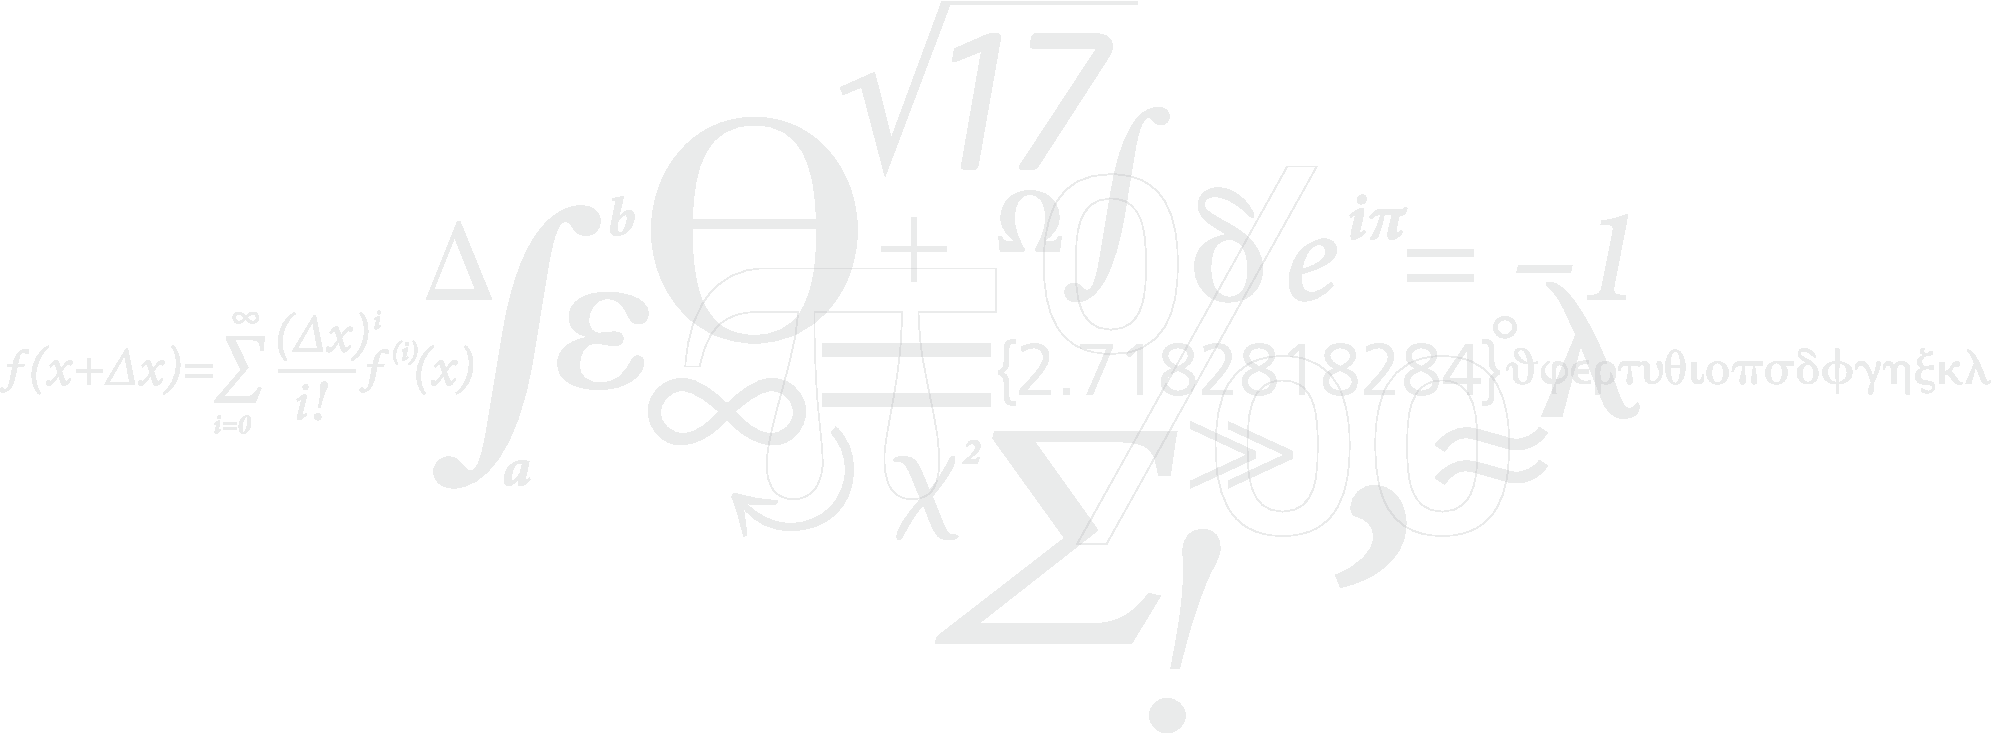
\includegraphics[trim=130mm 0 0 0,width=0.9\textwidth]{DTU-frise-SH-15}
                \vspace*{2.5cm}
            }
        }
    }
}

% This is a double sided book. If there is a last empty page lets use it for some fun e.g. the frieze.
% NB: For a fully functional hack the \clearpage used in \include does some odd things with the sequence numbering. Thefore use \input instead of \include at the end of the book. If bibliography is used at last everything should be ok.
\makeatletter
% Adjust so gatherings is allowd for single sheets too! (hacking functions in memoir.dtx)
\patchcmd{\leavespergathering}{\ifnum\@memcnta<\tw@}{\ifnum\@memcnta<\@ne}{
    \leavespergathering{1}
    % Insert the frieze
    \patchcmd{\@memensuresigpages}{\repeat}{\repeat\frieze{0}{0}}{}{}
}{}
\makeatother


% %% Sharelatex fix for microtype warnings
% \makeatletter
% \def\MT@is@composite#1#2\relax{%
%   \ifx\\#2\\\else
%     \expandafter\def\expandafter\MT@char\expandafter{\csname\expandafter
%                     \string\csname\MT@encoding\endcsname
%                     \MT@detokenize@n{#1}-\MT@detokenize@n{#2}\endcsname}%
%     % 3 lines added:
%     \ifx\UnicodeEncodingName\@undefined\else
%       \expandafter\expandafter\expandafter\MT@is@uni@comp\MT@char\iffontchar\else\fi\relax
%     \fi
%     \expandafter\expandafter\expandafter\MT@is@letter\MT@char\relax\relax
%     \ifnum\MT@char@ < \z@
%       \ifMT@xunicode
%         \edef\MT@char{\MT@exp@two@c\MT@strip@prefix\meaning\MT@char>\relax}%
%           \expandafter\MT@exp@two@c\expandafter\MT@is@charx\expandafter
%             \MT@char\MT@charxstring\relax\relax\relax\relax\relax
%       \fi
%     \fi
%   \fi
% }
% % new:
% \def\MT@is@uni@comp#1\iffontchar#2\else#3\fi\relax{%
%   \ifx\\#2\\\else\edef\MT@char{\iffontchar#2\fi}\fi
% }
% \makeatother\makeatother

%!TEX root = ../thesis.tex

% Text fonts (http://www.macfreek.nl/memory/Fonts_in_LaTeX)
% Install fonts from /usr/local/texlive/<version>/texmf-dist/fonts/opentype/public
\usepackage{fontspec}
\usepackage[T1]{fontenc}
\usepackage{lmodern}
\usepackage{slantsc}
% \RequirePackage{fix-cm}
\usepackage{bold-extra}
\usepackage{upgreek}

% \DeclareFontShape{T1}{texgyrepagella}{b}{sc}{<->ssub*cmr/bx/sc}{}
% \DeclareFontShape{T1}{texgyrepagella}{bx}{sc}{<->ssub*cmr/bx/sc}{}


% % Euler math fonts
% \usepackage[OT1,euler-digits,euler-hat-accent]{eulervm}
% \usepackage[bb=stixtwo]{mathalpha}
% \renewcommand{\mathbf}{\mathbold}  % euler requires \mathbold for bold math

% \usepackage{newtxmath}



% Serif font
% \usepackage{newpxtext}
% \setmainfont{TeX Gyre Pagella}
% \setmainfont{texgyrepagella}



\usepackage{mathpazo} % add possibly `sc` and `osf` options
\usepackage{eulervm}
\renewcommand{\mathbf}{\mathbold}  % euler requires \mathbold for bold math

% % Remove: "Font shape `T1/eulervm/m/n' undefined (Font) using `T1/cmr/m/n' instead."
% \usepackage{substitutefont}
% \substitutefont{TS1}{eulervm}{cmr}

%
% [
%   Extension=.otf,
%   UprightFont=*-regular,
%   ItalicFont=*-italic,
%   BoldFont=*-bold,
%   BoldItalicFont=*-bolditalic,
%   BoldSmallCapsFont=*-boldsmallcaps,
%   Numbers=OldStyle,
% ]

% \setmainfont{QTPalatine}

% \DeclareCharacterInheritance
%    { encoding = {TU,EU1,EU2},
%      family   = {QTPalatine} }
%    { A = {\`A,\'A,\^A,\~A,\"A,\r A},
%      a = {\`a,\'a,\^a,\~a,\"a,\r a},
%      C = {\c C},
%      c = {\c c},
%      D = {\DH},
%      d = {\dj},
%      E = {\`E,\'E,\^E,\"E},
%      e = {\`e,\'e,\^e,\"e},
%      I = {\`I,\'I,\^I,\"I},
%      i = {\`i,\'i,\^i,\"i,\i},
%      L = {\L},
%      l = {\l},
%      N = {\~N},
%      n = {\~n},
%      O = {\O,\`O,\'O,\^O,\~O,\"O},
%      o = {\o,\`o,\'o,\^o,\~o,\"o},
%      S = {\v S},
%      s = {\v s},
%      U = {\`U,\'U,\^U,\"U},
%      u = {\`u,\'u,\^u,\"u},
%      Y = {\'Y,\"Y},
%      y = {\'y,\"y},
%      Z = {\v Z},
%      z = {\v z}
%    }


% % Sans-serif font
% \setsansfont[
%     Ligatures=TeX,
%     Extension=.otf,
%     UprightFont=*-regular,
%     BoldFont=*-bold,
%     ItalicFont=*-italic,
%     BoldItalicFont=*-bolditalic,
%     % SlantedFont=,
%     % BoldSlantedFont=,
%     % SmallCapsFont=
%     Scale=0.8      % Adjustmens when using math in sections
% ]{texgyreadventor}


% Monospaced
% \setmonofont[Scale=MatchLowercase]{Linux Biolinum O}

%\setsansfont[Ligatures=TeX]{Neo Sans Intel}    % Neo Sans Intel – Like DTU font but more symbols
%\setsansfont[
%    Ligatures=TeX,
%    Scale=0.8
%]{NeoSans}           % NeoSans – DTU font (missing `+' symbols and other)
% \setsansfont[Ligatures=TeX]{CMU Sans Serif}    % Computer Modern Unicode font
%\setsansfont[Ligatures=TeX]{Latin Modern Sans} % Latin Modern Sans serif font

% Use this for more convienent sans serif font in math mode.
%\setmathsf{Latin Modern Sans}

%!TEX root = ../thesis.tex

% Content specific packages.

\usepackage{blindtext}
\usepackage{algorithm}
\usepackage{algpseudocode}
\usepackage{multicol}
\usepackage{multirow}
\usepackage{makecell}
\usepackage{booktabs}
\usepackage{enumerate}
\usepackage{enumitem}
% \usepackage{layouts}
\usepackage[showframe=\showframe,xetex]{geometry}
\usepackage{adjustbox}
\usepackage{siunitx}
\usepackage{nomencl}
\usepackage{amsmath}
\usepackage{amssymb}
\usepackage[acronym,toc]{glossaries}
%!TEX root = ../thesis.tex

% \makeglossaries
\makenoidxglossaries


% Glossary

\newglossaryentry{encoder}
{
    name=encoder,
    description={A general term for a function that maps an input to a different representation.}
}

\newglossaryentry{decoder}
{
    name=decoder,
    description={A general term for a function that maps a representation to an output.}
}


% Abbreviations
\newacronym{AI}{AI}{artificial intelligence}

\newacronym{MLP}{MLP}{multilayer perceptron}
\newacronym{FNN}{FNN}{feedforward neural network}
\newacronym{CNN}{CNN}{convolutional neural network}
\newacronym{RNN}{RNN}{recurrent neural network}
\newacronym{LSTM}{LSTM}{long short-term memory}
\newacronym{GRU}{GRU}{gated recurrent unit}
\newacronym{BNN}{BNN}{Bayesian neural network}

\newacronym{ReLU}{ReLU}{rectified linear unit}

\newacronym{SGD}{SGD}{stochastic gradient descent}

\newacronym{SGVB}{SGVB}{stochastic gradient variational Bayes}
\newacronym{VAE}{VAE}{variational autoencoder}
\newacronym{LVM}{LVM}{latent variable model}
\newacronym{KL}{KL}{Kullback-Leibler}

\newacronym{NLL}{NLL}{negative log-likelihood}
\newacronym{MSE}{MSE}{mean squared error}
\newacronym{CCE}{CCE}{categorical cross entropy}
\newacronym{MLE}{MLE}{maximum likelihood estimate}

\newacronym{PCA}{PCA}{principal components analysis}

\newacronym{PDF}{PDF}{probability density function}
\newacronym{PMF}{PMF}{probability mass function}

\newacronym{iid}{iid}{independent and identically distributed}

\newacronym{CPU}{CPU}{central processing unit}
\newacronym{GPU}{GPU}{graphics processing unit}
\newacronym{HPC}{HPC}{high performance computing}



%\usepackage{pgfplots}                 % Plot tools
%\pgfplotsset{compat=1.7}
\usetikzlibrary{
    arrows,
    matrix,
    positioning,
    shapes,
    shapes.multipart,
    topaths,
    bayesnet,
}
% tikzlibrary.code.tex
%
% Copyright 2010-2011 by Laura Dietz
% Copyright 2012 by Jaakko Luttinen
%
% This file may be distributed and/or modified
%
% 1. under the LaTeX Project Public License and/or
% 2. under the GNU General Public License.
%
% See the files LICENSE_LPPL and LICENSE_GPL for more details.

% Load other libraries
\usetikzlibrary{shapes}
\usetikzlibrary{fit}
\usetikzlibrary{chains}
\usetikzlibrary{arrows}

% Latent node
\tikzstyle{latent} = [circle,fill=white,draw=black,inner sep=1pt,
minimum size=20pt, font=\fontsize{10}{10}\selectfont, node distance=1]
% Observed node
\tikzstyle{obs} = [latent,fill=gray!25]
% Constant node
\tikzstyle{const} = [rectangle, inner sep=0pt, node distance=1]
% Factor node
\tikzstyle{factor} = [rectangle, fill=black,minimum size=5pt, inner
sep=0pt, node distance=0.4]
% Deterministic node
\tikzstyle{det} = [latent, diamond]

% Plate node
\tikzstyle{plate} = [draw, rectangle, rounded corners, fit=#1]
% Invisible wrapper node
\tikzstyle{wrap} = [inner sep=0pt, fit=#1]
% Gate
\tikzstyle{gate} = [draw, rectangle, dashed, fit=#1]

% Caption node
\tikzstyle{caption} = [font=\footnotesize, node distance=0] %
\tikzstyle{plate caption} = [caption, node distance=0, inner sep=0pt,
below left=5pt and 0pt of #1.south east] %
\tikzstyle{factor caption} = [caption] %
\tikzstyle{every label} += [caption] %

\tikzset{>={triangle 45}}

%\pgfdeclarelayer{b}
%\pgfdeclarelayer{f}
%\pgfsetlayers{b,main,f}

% \factoredge [options] {inputs} {factors} {outputs}
\renewcommand{\factoredge}[4][]{ %
  % Connect all nodes #2 to all nodes #4 via all factors #3.
  \foreach \f in {#3} { %
    \foreach \x in {#2} { %
      \path (\x) edge[-,#1] (\f) ; %
      %\draw[-,#1] (\x) edge[-] (\f) ; %
    } ;
    \foreach \y in {#4} { %
      \path (\f) edge[->,#1] (\y) ; %
      %\draw[->,#1] (\f) -- (\y) ; %
    } ;
  } ;
}

% \edge [options] {inputs} {outputs}
\renewcommand{\edge}[3][]{ %
  % Connect all nodes #2 to all nodes #3.
  \foreach \x in {#2} { %
    \foreach \y in {#3} { %
      \path (\x) edge [->,#1] (\y) ;%
      %\draw[->,#1] (\x) -- (\y) ;%
    } ;
  } ;
}

% \factor [options] {name} {caption} {inputs} {outputs}
\renewcommand{\factor}[5][]{ %
  % Draw the factor node. Use alias to allow empty names.
  \node[factor, label={[name=#2-caption]#3}, name=#2, #1,
  alias=#2-alias] {} ; %
  % Connect all inputs to outputs via this factor
  \factoredge {#4} {#2-alias} {#5} ; %
}

% \plate [options] {name} {fitlist} {caption}
\renewcommand{\plate}[4][]{ %
  \node[wrap=#3] (#2-wrap) {}; %
  \node[plate caption=#2-wrap] (#2-caption) {#4}; %
  \node[plate=(#2-wrap)(#2-caption), #1] (#2) {}; %
}

% \gate [options] {name} {fitlist} {inputs}
\renewcommand{\gate}[4][]{ %
  \node[gate=#3, name=#2, #1, alias=#2-alias] {}; %
  \foreach \x in {#4} { %
    \draw [-*,thick] (\x) -- (#2-alias); %
  } ;%
}

% \vgate {name} {fitlist-left} {caption-left} {fitlist-right}
% {caption-right} {inputs}
\renewcommand{\vgate}[6]{ %
  % Wrap the left and right parts
  \node[wrap=#2] (#1-left) {}; %
  \node[wrap=#4] (#1-right) {}; %
  % Draw the gate
  \node[gate=(#1-left)(#1-right)] (#1) {}; %
  % Add captions
  \node[caption, below left=of #1.north ] (#1-left-caption)
  {#3}; %
  \node[caption, below right=of #1.north ] (#1-right-caption)
  {#5}; %
  % Draw middle separation
  \draw [-, dashed] (#1.north) -- (#1.south); %
  % Draw inputs
  \foreach \x in {#6} { %
    \draw [-*,thick] (\x) -- (#1); %
  } ;%
}

% \hgate {name} {fitlist-top} {caption-top} {fitlist-bottom}
% {caption-bottom} {inputs}
\renewcommand{\hgate}[6]{ %
  % Wrap the left and right parts
  \node[wrap=#2] (#1-top) {}; %
  \node[wrap=#4] (#1-bottom) {}; %
  % Draw the gate
  \node[gate=(#1-top)(#1-bottom)] (#1) {}; %
  % Add captions
  \node[caption, above right=of #1.west ] (#1-top-caption)
  {#3}; %
  \node[caption, below right=of #1.west ] (#1-bottom-caption)
  {#5}; %
  % Draw middle separation
  \draw [-, dashed] (#1.west) -- (#1.east); %
  % Draw inputs
  \foreach \x in {#6} { %
    \draw [-*,thick] (\x) -- (#1); %
  } ;%
}



\definecolor{customgreen} {RGB}{217	234	212}
\definecolor{customblue}  {RGB}{205	226	242}
\definecolor{custommorered}{RGB}{218 46 42}
\definecolor{customred}{RGB}{255 182 173}%{255 149 150}

\colorlet{observed-color}{customgreen}
\colorlet{latent-color}{customblue}
\colorlet{deterministic-color}{gray!15}
\colorlet{deterministic-skip-color}{custommorered}
\colorlet{shared-function-color}{blue}


% Listings
\lstset{
    basicstyle=\footnotesize\ttfamily,% the size of the fonts that are used for the code
    breakatwhitespace=false,          % sets if automatic breaks should only happen at whitespace
    breaklines=true,                  % sets automatic line breaking
    captionpos=b,                     % sets the caption-position to bottom
    commentstyle=\color{s14a},        % comment style
    deletekeywords={},                % if you want to delete keywords from the given language
    escapeinside={\%*}{*)},           % if you want to add LaTeX within your code
    frame=single,                     % adds a frame around the code
    keywordstyle=\bfseries\ttfamily\color{s09}, % keyword style
    language=Python,                  % the language of the code
    morekeywords={*,...},             % if you want to add more keywords to the set
    numbers=left,                     % where to put the line-numbers; possible values are (none, left, right)
    numbersep=5pt,                    % how far the line-numbers are from the code
    numberstyle=\sffamily\tiny\color{dtugray}, % the style that is used for the line-numbers
    rulecolor=\color{dtugray},        % if not set, the frame-color may be changed on line-breaks within not-black text (e.g. comments (green here))
    showspaces=false,                 % show spaces everywhere adding particular underscores; it overrides 'showstringspaces'
    showstringspaces=false,           % underline spaces within strings only
    showtabs=false,                   % show tabs within strings adding particular underscores
    stepnumber=1,                     % the step between two line-numbers. If it's 1, each line will be numbered
    stringstyle=\color{s07},          % string literal style
    tabsize=2,                        % sets default tabsize to 2 spaces
    title=\lstname,                   % show the filename of files included with \lstinputlisting; also try caption instead of title
}



\addbibresource{bibliography/zotero-references.bib}

\begin{document}

\prefrontmatter
%!TEX root = ../thesis.tex 

\thispagestyle{empty}             % No page numbers
\calccentering{\unitlength}
\begin{adjustwidth*}{\unitlength}{-\unitlength}
    \begin{adjustwidth}{-0.5cm}{-0.5cm}
        \scshape
        % \MakeUppercase
        \begin{flushright}
            \scriptsize  % \fontsize{10}{10}\selectfont
            \def\arraystretch{1.2}
            \begin{tabular}{rc}
            & \multirow{4}{*}{
\includegraphics[height=1.5cm]{DTU-logo-CMYK}}\\[-0.1cm]
            \thesistypeabbr{} Thesis & \\
            \thesistype{} & \\
            Technical University of Denmark &
            \end{tabular}        
        \end{flushright}
        % \begin{flushright}
        %     \small
        %     \thesistypeabbr{} Thesis\\*[0cm]
        %     \thesistype{}\\
        %     
\includegraphics[scale=0.7]{DTU-logo-CMYK}
        % \end{flushright}
        \vspace*{\fill}
        \begin{center}
        {\color{dtured}\noindent\large\thesistitle}\\*[0.2cm]
        \large{\thesissubtitle}\\*[1.2cm]
        % \parbox[b]{0.5\linewidth}{%
            \normalsize
            \thesisauthor\\*[1.2cm]
            % \thesislocation{}\\*[0.5cm]
            \thesismonth\ \thesisyear, \thesislocation
        % }
        \end{center}
        \vspace*{\fill}
        % 
\includegraphics[width=0.75\textwidth]{DTU-Compute-B-UK}\\*[0.5cm]
        % \normalsize
        % \vspace{1.2cm}
        % \begin{tabular}{d{1mm}l}
        % \thesisdepshort \\
        % {\color{dtugray!150}\thesisdep}
        % \end{tabular}
    \end{adjustwidth}
\end{adjustwidth*}
\normalfont
\normalsize

\cleartoevenpage
%!TEX root = ../thesis.tex

\thispagestyle{empty} % No page numbers
\frieze{0}{0.5\paperheight}

\vspace*{\fill}
% \vspace*{0.15\textheight}
\small%\sffamily
\noindent
\textsc{\textbf{Technical University of Denmark}}\\
\textsc{\textbf{Department of Applied Mathematics and Computer Science}}
\smallskip\\
\href{https://goo.gl/maps/Dx6rNjGT9Ad5xKgZ6}{%
Richard Petersens Plads, Building 324\\
2800 Kongens Lyngby, Denmark}\\
% Phone +45 4525 3031\\
\href{mailto:compute@compute.dtu.dk}{compute@compute.dtu.dk}\\
\href{www.compute.dtu.dk}{www.compute.dtu.dk}
\bigskip\\
\noindent
\textsc{\textbf{Corti}}\\
\textsc{\textbf{Department for Research and Development}}
\smallskip\\
\href{https://goo.gl/maps/X7en4p8vaHkfVuyJ7}{%
Store Strandstræde 21. 4.\\
1255 København K, Denmark}\\
\href{mailto:info@corti.ai}{info@corti.ai}\\
\href{www.corti.ai}{www.corti.ai}\\

\normalsize
\normalfont
\cleartooddpage
%!TEX root = ../thesis.tex
% \chapter*{Supervision}

\thispagestyle{empty} % No page numbers

\hfill\vfill

\noindent
\sffamily
\textsc{\textbf{Academic supervision}}
\medskip
\\Jes Frellsen\\
\textit{Supervisor, Technical University of Denmark}
\medskip
\\Søren Hauberg\\
\textit{Co-supervisor, Technical University of Denmark}
\medskip
\\Ole Winther\\
\textit{Co-supervisor, Technical University of Denmark}
\medskip

\bigskip
\noindent
\textsc{\textbf{Industrial supervision}}
\medskip
\\Lars Maaløe\\
\textit{Supervisor, Corti \& Technical University of Denmark}
\medskip
\\Željko Agi\'c\\
\textit{Co-supervisor, Unity Technologies}
\medskip

\bigskip
\noindent
\textsc{\textbf{Assessment committee}}
\medskip
\\Person 1\\
\textit{University of Copenhagen}
\medskip
\\Person 2\\
\textit{Toyota Technological Institute at Chicago}
\medskip
\\Person 3\\
\textit{Carnegie Mellon University}
\medskip

\bigskip
\noindent
\textsc{\textbf{Author}}
\medskip
\\\thesisauthor\\
\textit{Technical University of Denmark \& Corti}\\
\thesistypeabbr\ thesis\\
\textit{\thesistitle}\\
\textcopyright\ \thesismonth\ \thesisyear

\normalsize
\normalfont

% \clearforchapter
\cleartoevenpage

\frontmatter
%!TEX root = ../thesis.tex


% Ph.D. Bekendtgørelsen
% Bekendtgørelse om ph.d.-uddannelsen ved universiteterne og visse kunstneriske uddannelsesinstitutioner
% https://www.retsinformation.dk/eli/lta/2013/1039
%
% Universitetsloven
% Bekendtgørelse af lov nr. 778 af 7. august 2019 om universiteter
% https://www.retsinformation.dk/eli/lta/2019/778

\chapter*[declaration]{Declaration}
\thispagestyle{empty}
This \thesistypeabbr\ thesis was prepared at the \thesisdep\ at the Technical University of Denmark in fulfillment of the requirements for acquiring a \thesistypeabbr\ degree.
\bigskip
 
\noindent\textit{\thesislocation, \thesismonth\ \thesisday,\ \thesisyear}

\smallskip

\begin{flushright}
    \renewcommand{\arraystretch}{0.5}
    \begin{tabular}{c}
        
\includegraphics[width=0.3\textwidth]{graphics/signature.pdf} \\
        \rule{0.4\textwidth}{0.4pt} \\
        \\
        \thesisauthor \\
    \end{tabular}
    \hspace*{0.05\textwidth}
\end{flushright}



% \begin{flushright}
%     \begin{tabular}{m{0.4\textwidth}}
%         \\ 
\includegraphics[scale=0.1]{graphics/signature.pdf} \ \\ %
%         \\ \hline \\
%         \vspace{1pt}\centering\thesisauthor \\
%     \end{tabular}
%     \hspace*{0.05\textwidth}
% \end{flushright}

%!TEX root = ../thesis.tex

\chapter[abstract]{Abstract}

Natural language plays a pivotal role in patient interactions within healthcare systems worldwide. Despite significant advancements in medicine and medical technology, patient interviews and general medical communication have remained largely unchanged. Typically, a single healthcare professional, whether a medical helpline operator, paramedic, general practitioner, or medical coder, is tasked with understanding patient needs and taking appropriate action. With aging populations, expanding treatment options, administrative burdens, and strict documentation requirements, healthcare professionals face mounting pressure in an increasingly complex environment. These challenges pose risks to staff retention, quality of care, and the potential for medical errors.

Machine learning presents an opportunity to support healthcare professionals in different medical settings, including primary care clinics and emergency services. Previous machine learning applications in healthcare have often neglected natural language, focusing on tasks involving structured data like predicting medical imaging outcomes and analyzing electronic health records. However, the utilization of machine learning systems to interpret natural language can alleviate the administrative and documentation burdens on healthcare professionals and help ensure that critical information is not overlooked or forgotten.

Developing machine learning systems for medical conversations is challenging due to the high-stakes nature of healthcare decisions and the complexity of unstructured language data, including speech and text. While neural network-based machine learning systems have demonstrated impressive performance in other domains, their application in healthcare can be hindered by interpretability issues and their poor ability to quantify predictive uncertainty, particularly in dynamic environments and for rare cases commonly referred to as out-of-distribution data.

This thesis explores machine learning techniques for medical conversations, with a primary focus on uncertainty estimation and natural language processing. The first part investigates unsupervised methods for detecting out-of-distribution data and modeling speech using variational autoencoders, making the following contributions:
%
\begin{enumerate}[label=(\roman*)] 
    \item Empirical and theoretical evidence which demonstrates that low-level features dominate the likelihood estimate of hierarchical variational autoencoders and impedes detection of out-of-distribution data, as well as a novel likelihood-ratio score that requires data to be in-distribution across all feature levels.
    % \item A novel likelihood-ratio score for unsupervised out-of-distribution detection with hierarchical variational autoencoders that requires data to be in-distribution across all feature-levels. 
    \item A model-agnostic statistical test employing Fisher's method to combine Rao's score test and the recently introduced typicality test, applicable with likelihoods from any differentiable generative model.
    \item Demonstrated improvements in likelihoods on speech data and latent spaces that capture information relevant for speech by using hierarchical variational autoencoders compared to shallow variants.
\end{enumerate}
%
The second part of this thesis explores self-supervised methods for speech representation and comprehension and contributes with:
%
\begin{enumerate}[resume, label=(\roman*)] 
    \item A comprehensive review of self-supervised speech representation learning that categorizes methods into contrastive, autoregressive, and generative approaches, provides a comparison of training objectives, model architectures, and downstream task performance, and discusses promising future research directions.
\end{enumerate}
%
The final part centers on medical applications of machine learning and makes the following contributions:
%
\begin{enumerate}[resume, label=(\roman*)] 
    \item An analysis of state-of-the-art models for automated medical coding on MIMIC-III and IV datasets. This analysis identifies suboptimal training practices, evaluation methods, and non-stratified data splits as factors contributing to poor performance. It subsequently presents a revised comparison using improved data splits and identical experimental setups shedding light on the true comparative performance of the methods.
    \item A retrospective study demonstrating that an audio-based machine learning framework can significantly improve stroke recognition in calls made to the prehospital medical helpline, 1813, serving the Copenhagen area.
\end{enumerate}
%
In summary, this thesis advances the field of machine learning in healthcare by addressing challenges in natural language processing, uncertainty estimation, and medical applications which might ultimately contribute to improved patient care and clinical decision-making.

%!TEX root = ../thesis.tex
% LTeX: language=da-DK

\chapter[resumé (abstract in danish)]{Resumé (Abstract in Danish)}

Naturligt sprog spiller en nøglerolle i sundhedssystemer verden over. Alligevel har den medicinske interviewproces kun oplevet en lille udvikling sammenlignet fremskridtene inden for medicinsk teknologi.
Traditionelt udføres medicinske interviews af sundhedspersonale, der primært afhænger af deres individuelle erfaring for at forstå en situation.
Med aldrende befolkninger, strenge dokumentationskrav, og fremskridt inden for diagnostiske muligheder og behandlingsmuligheder, er denne tilgang dyr og risikerer at komme til kort, hvilket potentielt kompromitterer nøjagtigheden og kvaliteten af medicinsk behandling.

Nylige fremskridt inden for naturlig sprogbehandling gør det muligt for maskinlæringsmodeller at deltage aktivt i medicinske interviews for at lette administrative byrder, forbedre dokumentation, og assistere i realtid.
Sundhedsplejen adskiller sig dog fra andre domæner på grund af den høje risiko forbundet med selv små fejl. Da ingen model er fejlfri, tilskynder dette til at associere modelprædiktioner med robuste usikkerhedsestimater, især i scenarier, der involverer ude-af-fordeling (UAF) data, såsom sjældne sygdomme.

Denne afhandling tager udgangspunkt i hovedhypotesen, at usuperviseret repræsentationslæring er nyttig til usikkerhedsestimering i medicinske opgaver.
Den giver følgende bidrag:
%
\begin{enumerate}[topsep=3pt, partopsep=0pt, itemsep=3pt, parsep=0pt, leftmargin=2em, label=(\alph*)] %, label=(\roman*)]
    \item En likelihood-ratio score til UAF-detektion med variationelle autoenkodere, der afhjælper den bevist negative effekt af lav-niveau features.
    \item En statistisk test til UAF-detektion, der kombinerer score- og typikalitetstests og kan bruges med likelihoods fra enhver differentiabel generativ model.
    \item Et benchmark for probabilistiske talerepræsentationsmodeller og en ny metode til at lære hierarkiske repræsentationer.
    \item En oversigt over usuperviseret repræsentationslæring til neural talebehandling og en tilsvarende modeltaksonomi.
    \item En fejlanalyse og revideret evaluering af state-of-the-art modeller til automatiseret medicinsk kodning på MIMIC-III og IV datasættene.
    \item Et retrospektivt studie af talebaseret genkendelse af stroke i præhospitale akuttelefonopkald der viser betydelig forbedring i forhold til opkaldstagere.
\end{enumerate}
%

Sammenfattende adresserer denne afhandling udfordringer indenfor usikkerhedsestimering og repræsentationslæring til tale og udforsker medicinske anvendelser af maskinlæring. 
Dens bidrag er afgørende i udviklingen af et operationelt beslutningsstøttesystem til medicinske interviews, der søger at øge kvaliteten af patientbehandlingen ved at understøtte effektiv, informeret beslutningstagen.

%!TEX root = ../thesis.tex

\chapter[publications]{Publications}

This thesis consists of the following papers which are categorized as either \textsc{primary} and \textsc{secondary}. 
Each \textsc{primary} paper makes up a chapter of the thesis while \textsc{secondary} papers are included in the appendix. 
Published papers have been reformatted to fit the layout, but the content has not been changed. 

\vspace{5mm}

\raggedright\par\noindent\hspace{8mm}{\large\scshape primary}\\[-2mm]

\raggedleft\rule{\textwidth - 8mm}{0.4pt}

\begin{enumerate}[leftmargin=8mm,topsep=0mm,label={[\Alph*]}]

    \item \fullcite{havtorn_hierarchical_2021}
    \item \fullcite{havtorn_benchmarking_2022} 
    \item \fullcite{mohamed_selfsupervised_2022}
    % \item \fullcite{havtorn_uncertainty_for_asr_2023}
    % \item \fullcite{wenstrup_ml_for_stroke_2023}

\end{enumerate}

\vspace{5mm}

\raggedright\par\noindent\hspace{8mm}{\large\scshape secondary}\\[-2mm]

\raggedleft\rule{\textwidth - 8mm}{0.4pt}

\begin{enumerate}[leftmargin=8mm,topsep=0mm,label={[\Alph*]}]
    \setcounter{enumi}{2}

    \item \fullcite{borgholt_endtoend_2020}
    \item \fullcite{havtorn_multiqt_2020}
    \item \fullcite{borgholt_scaling_2021}
    \item \fullcite{borgholt_we_2021}
    \item \fullcite{borgholt_brief_2022}

\end{enumerate}

% \raggedright

\justifying

\vspace*{\fill}

%!TEX root = ../thesis.tex

\chapter[acknowledgements]{Acknowledgements}
First, I want to thank my supervisors. Jes, you have been an amazing support through this project. 
Your positivity and insightfulness were essential to me daring to take on this project, and to its success. 
Lars, you have been a completely indispensable source of purpose, energy, and direction throughout my time with Corti. I look forward to many more fruitful discussions in the future.

I also want to thank the brilliant researchers at the section for Cognitive Systems that I have had the privilege of working with. 
Søren, as my co-supervisor, you have been a fantastic discussion partner. Your wit and your ability to pose genuinely significant questions have been invaluable. 
I want to also convey appreciation for the researchers in my group, for the open, inclusive, and relaxed culture, and for many good discussions, often over coffee and pastries.

I want to thank Lars, Andreas, and Michael for letting me become part of the Corti project after graduating back in 2018. 
The foundational will to invest and believe in people, and to dare to have bold visions, has made Corti a fantastic place for me to develop, professionally and personally. 
I want to also thank the members of the machine learning team during the first years of my time at Corti. Lasse, Tycho, Marco, Jan, Janek, and Joakim, you all played a part in inspiring and enabling me to dive into this project. 
A special thanks should go to Joakim. Your honest curiosity and dedication has been a wonderful addition to the research team. 
I also want to thank Lasse. The numerous inspirational discussions with you and our combined efforts through the years have been instrumental in shaping this thesis. It has been a privilege to carry out this PhD project in the company of you both. 

I want to also thank my friends and my family who have provided much needed diversion and encouragement throughout the years. 
Last, but not least, I want to thank my wife, Rikke, who has been an unbelievably patient and absolutely essential supporter at every step of this undertaking. I am excited about what lies ahead for us and our daughter Vigga, and I cannot wait to build our future together. 

\vspace*{\fill}
\noindent \textit{The project was funded by Corti and Innovation Fund Denmark through industrial PhD grant no.\@ 0153-00167B.}

%     %!TEX root = ../thesis.tex

\makenomenclature
%\markboth{\MakeUppercase\nomname}{\MakeUppercase\nomname}

% Correct header on multiple page nomenclature
\patchcmd{\thenomenclature}
  {\chapter*{\nomname}}% usually only \chapter*{\nomname} is issued
  {\chapter*{\nomname}\markboth{\MakeUppercase\nomname}{\MakeUppercase\nomname}}
  {}{}

\renewcommand{\nomname}{Notation}  % Rename Nomenclature to Notation

\setlength{\nomlabelwidth}{3cm}  % Increase width of box for mathematical symbol on left
% \setlength{\nomitemsep}{-\parsep}

% Command for the group subtitles
\newcommand{\nommenclaturesubtitle}[1]{%
    \bigskip
    \item[\bfseries \hspace{3cm}\: #1
        % \vspace{1cm}\\
        % \hspace{2.4cm} #1 \hfill\\
        % \par\noindent\rule{\widthof{#1}}{1pt}
    ]
    %\par\noindent\rule{\widthof{#1}}{1pt}%
    %   \hspace*{-\leftmargin}%
    %   \rule[2pt]{0.45\linewidth}{1pt}%
    %   \hfill #1\hfill
    %   \rule[2pt]{0.45\linewidth}{1pt}%
}

% Introductory text to notation section
\renewcommand{\nompreamble}{%
    This section collects definitions of the notation used in the thesis. Much of this is defined in the thesis in the order that it is used but is collected here for reference and convenience. There are no major departures from convention.
}

% Definition of the groups
\renewcommand\nomgroup[1]{%
      \ifstrequal{#1}{A}{\nommenclaturesubtitle{Numbers and arrays}}{%
      \ifstrequal{#1}{B}{\nommenclaturesubtitle{Sets}}{%
      \ifstrequal{#1}{C}{\nommenclaturesubtitle{Indexing}}{%
      \ifstrequal{#1}{D}{\nommenclaturesubtitle{Linear algebra operations}}{%
      \ifstrequal{#1}{E}{\nommenclaturesubtitle{Calculus}}{%
      \ifstrequal{#1}{F}{\nommenclaturesubtitle{Probability theory}}{%
      \ifstrequal{#1}{G}{\nommenclaturesubtitle{Functions}}{%
      }}}}}}}
}

% Notation entries
\nomenclature[A, 01]{$a$}{A scalar; integer or real}
\nomenclature[A, 02]{$\ab$}{A column vector}
\nomenclature[A, 03]{$\Ab$}{A matrix}
\nomenclature[A, 04]{$\text{diag}(\ab)$}{A square diagonal matrix of the elements of $\ab$}
\nomenclature[A, 05]{$\e$}{A vector of ones, $\e=\bmat{1 & \cdots & 1}\transpose$}
\nomenclature[A, 06]{$\Ib$}{The identity matrix, $\Ib=\text{diag}\pa{\e}$}

\nomenclature[B, 01]{$\mathcal{A}, \mathbb{A}$}{A set}
\nomenclature[B, 02]{$\mathbb{R}$}{Set of real numbers}
\nomenclature[B, 03]{$\cbra{s_1, s_2, \dots, s_n}$}{Set of scalars $s_1, s_2, \dots, s_n$; also written as $\cbra{s_i}_{i=1}^n$}
%\nomenclature[B, 04]{$\bra{a, b}$}{Inclusive real interval between $a$ and $b$, $\bra{a, b}=\cbra{x\in\mathbb{R}\mid a\leq x \leq b}$}
%\nomenclature[B, 05]{$\pa{a, b}$}{Exclusive real interval between $a$ and $b$, $\pa{a, b}=\cbra{x\in\mathbb{R}\mid a<x<b}$}
\nomenclature[B, 06]{$\left(a, b\right]$}{Semi-inclusive real interval between $a$ and $b$, $\left(a, b\right]=\cbra{x\in\mathbb{R}\mid a<x\leq b}$}

\nomenclature[C, 01]{$a_i$}{Element $i$ of vector $\ab$ with first index $1$}
\nomenclature[C, 02]{$A_{i,j}$}{Element $i,j$ of matrix $\Ab$. Comma omitted when unambiguous.}
\nomenclature[C, 03]{$A_{i,:}$}{Row $i$ of matrix $\Ab$ (a row vector)}
\nomenclature[C, 04]{$A_{:,j}$}{Column $j$ of matrix $\Ab$ (a column vector)}
\nomenclature[C, 05]{$\ab^\bra{l}$}{Neural network layer indexing; a vector in layer $l$}
\nomenclature[C, 06]{$\ab^\vbra{t}$}{Recurrent neural network sequence indexing; vector at timestep $t$ in sequence $\cbra{\ab^\vbra{t}}_{t=1}^T$}

\nomenclature[D, 01]{$\ab\transpose$}{Transpose of column vector $\ab$ to give row vector}
\nomenclature[D, 02]{$\Ab\transpose$}{Transpose of matrix $\Ab$}
\nomenclature[D, 03]{$\ab\transpose\bb$}{Inner product of $\ab$ and $\bb$, $\ab\transpose\bb=\ab\cdot\bb$}
\nomenclature[D, 04]{$\ab\bb\transpose$}{Outer product of $\ab$ and $\bb$}
\nomenclature[D, 05]{$\Ab\Bb$}{Matrix product of $\Ab$ and $\Bb$}
\nomenclature[D, 06]{$\Ab*\Bb$}{Convolution (actually cross-correlation) of $\Ab$ and $\Bb$}
\nomenclature[D, 07]{$\Ab\odot\Bb$}{Elementwise, or Hadamard, product of $\Ab$ and $\Bb$}
\nomenclature[D, 08]{$\det{\Ab}$}{Determinant of matrix $\Ab$}
\nomenclature[D, 09]{$\norm{\ab}$}{$L^2$ norm of $\ab$}
\nomenclature[D, 10]{$\norm{\ab}_p$}{$L^p$ norm of $\ab$}
\nomenclature[D, 11]{$\Tr{\Ab}$}{Trace of matrix $\Ab$, $\Tr{\Ab}=\sum_i A_{i,i}$}

\nomenclature[E, 01]{$\frac{\text{d}y}{\text{d}x}$}{Derivative of $y$ with respect to $x$}
\nomenclature[E, 02]{$\pd{y}{x}$}{Partial derivative of $y$ with respect to $x$}
\nomenclature[E, 03]{$\nabla_\xb$}{Del, nabla or Laplacian operator, $\nabla_\xb = \bmat{\pd{}{x_1} & \cdots & \pd{}{x_n}}^\text{T}, \; \xb\in\mathbb{R}^{n}$}
\nomenclature[E, 04]{$\nabla_\xb y$}{Gradient of $y$ with respect to $\xb$, $\nabla_\xb y = \bmat{\pd{y}{x_1} & \cdots & \pd{y}{x_n}}^\text{T}, \; \xb\in\mathbb{R}^{n}$}
\nomenclature[E, 05]{$\Hb_\xb$}{Hessian operator, $\Hb_\xb = \nabla_\xb\nabla_\xb\transpose = \bmat{
	    \pd[2]{}{x_1} & \frac{\partial^2}{\partial x_1 \partial x_2} & \cdots & \frac{\partial^2}{\partial x_1 \partial x_n}\\
	    \frac{\partial^2}{\partial x_2 \partial x_1} & \pd[2]{}{x_2} & \cdots & \frac{\partial^2}{\partial x_2 \partial x_n}\\
	    \vdots & \vdots & \ddots & \vdots\\
	    \frac{\partial^2}{\partial x_n \partial x_1} & \frac{\partial^2}{\partial x_n \partial x_2} & \cdots & \pd[2]{}{x_n}
	    }$}
\nomenclature[E, 06]{$\Hb_\xb y$}{Hessian matrix of $y$ with respect to $\xb$; matrix of all second order partial derivatives}
\nomenclature[E, 07]{$\nabla^2_\xb$}{Laplacian operator, $\nabla^2_\xb=\nabla_\xb\transpose\nabla_\xb = \nabla_\xb\cdot\nabla_\xb=\sum_i \pd[2]{}{x_i}=\Tr{\Hbb_\xb}$}
\nomenclature[E, 08]{$\nabla^2_\xb y$}{Laplacian of $y$ with respect to $\xb$; sum of the unmixed second order partial derivatives}
\nomenclature[E, 09]{$\pd{\y}{\xb}$}{Jacobian matrix of $\y$ w.r.t. $\xb$, $\pd{\y}{\xb} = \bmat{
	    \nabla_\xb y_1 &
	    \cdots &
	    \nabla_x y_n}^\text{T}, \; \y\in\mathbb{R}^{n}$; matrix of all possible first order partial derivatives}
\nomenclature[E, 10]{$\int f(\xb)\,\text{d}\xb$}{Definite integral over the domain of $\xb$}
\nomenclature[E, 11]{$\int_\mathcal{D} f(\xb)\,\text{d}\xb$}{Definite integral over the domain $\mathcal{D}$}

\nomenclature[F, 01]{$a\sim p$}{$a$ is a random variable with distribution $p$}
\nomenclature[F, 02]{$\text{E}\bra{f(x)}$}{Expectation of $f(x)$ with respect to $p(x)$; sometimes also $\text{E}\bra{f(x)}_{x\sim p(x)}$}
\nomenclature[F, 03]{$\text{Var}\bra{f(x)}$}{Variance of $f(x)$ under $p(x)$}
\nomenclature[F, 04]{$\text{Cov}\bra{f(x), g(x)}$}{Covariance of $f(x)$ and $g(x)$ under $p(x)$}
\nomenclature[F, 05]{$D_\text{KL}\pa{p\mid\mid q}$}{Kullback-Leibler divergence of $p$ and $q$}
\nomenclature[F, 06]{$D_\text{KL}\pa{p,q}$}{Symmetrized Kullback-Leibler divergence of $p$ and $q$}
\nomenclature[F, 07]{$\mathcal{N}\pa{\xb\mid\mub,\Sigmab}$}{Gaussian distribution over $\xb$ with mean $\mub$ and covariance $\Sigmab$}

\nomenclature[G, 01]{$f:\mathcal{D}\rightarrow\mathcal{C}$}{Function $f$ with domain $\mathcal{D}$ and co-domain $\mathcal{C}$}
\nomenclature[G, 02]{$\log x$}{Natural logarithm of $x$}
\nomenclature[G, 03]{$\text{ReLU}\pa{x}$}{Linear rectifier function, $\text{ReLU}\pa{x}=\max\cbra{0,x}$ (Rectified Linear Unit)}


\clearforchapter
\printglossary[title=Abbreviations, toctitle=abbrevations, type=\acronymtype]
\clearforchapter
\tableofcontents*
\clearforchapter
\mylistoftodos

\mainmatter
\part[introduction and background]{introduction and background}
\chapter[introduction]{Introduction}

Introduction with some math $x^2 = \prod_{i=1}^{2} x$ and some stuff.

$$
p(x) = \mathcal{N}(x; \mu, \sigma^2)
$$


\chapter[background]{Background}

\cite{bahdanau_neural_2014}

\part[discussion and conclusions]{discussion and conclusions}
%!TEX root = ../thesis.tex
\chapter[conclusion]{Conclusion}
A conclusion with some abbreviations and citations, \gls{VAE} \cite{kingma_autoencoding_2014,rezende_stochastic_2014}.



% %!TEX root = ../thesis.tex
\chapter{Introduction}

\begin{itemize}
    \item \textup{Upright shape}
    \item \textit{Italic shape}
    \item \textsl{Slanted shape}
    \item \textsc{Small Caps shape}
    \item \textmd{Medium series}
    \item \textbf{Bold sereies}
    \item \textrm{Roman family}
    \item \textsf{Sans serif family}
    \item \texttt{Typewriter family}
\end{itemize}

I love to write special characters like øæå indside my \TeX{} document. Also á, à, ü, û, ë, ê, î, ï could be nice. So waht about the ``π'' chracter. What about ° é ® † ¥ ü | œ π ‘ @ ö ä ¬ ∆ ‹ « © ƒ ∂ ß ª Ω … ç √ ∫ ñ µ ‚ · ¡ “ £ ∞ ™ [ ] ≠ ± '.

Some dashes - – —, and the latex form - -- ---
\begin{equation*}
    x = \mathtt{x}, \mathbf{x}, \mathit{x}, x_{1_{2_{3_{4}}}}^{1^{2^{3^{4}}}} \cdot hello * \text{hello world} ⋅ \text{my world} · \text{third world} ⊗ t
\end{equation*}

Lorem ipsum dolor sit amet, consectetur adipisicing elit, sed do eiusmod tempor incididunt ut labore et dolore magna aliqua. Ut enim ad minim veniam, quis nostrud exercitation ullamco laboris nisi ut aliquip ex ea commodo consequat. Duis aute irure dolor in reprehenderit in voluptate velit esse cillum dolore eu fugiat nulla pariatur. Excepteur sint occaecat cupidatat non proident, sunt in culpa qui officia deserunt mollit anim id est laborum \parencite{adams1980hitchhiker}.

Mauris id quam non magna fermentum malesuada id mattis lorem. In a dapibus neque. Etiam lacus dui, malesuada ac eleifend imperdiet, imperdiet ut ipsum. Vestibulum id ultricies est. Phasellus augue mauris, semper a luctus vel, faucibus in risus. Fusce commodo augue quis elit sagittis non viverra turpis bibendum. Nunc placerat sem non sapien malesuada malesuada ullamcorper orci luctus \parencite{adams1980hitchhiker}. Morbi pharetra ligula integer mollis mi nec neque ultrices vitae volutpat leo ullamcorper. In at tellus magna. Curabitur quis posuere purus. Cum sociis natoque penatibus et magnis dis parturient montes, nascetur ridiculus mus. Suspendisse tristique placerat feugiat. Aliquam vitae est at enim auctor ultrices eleifend a urna. Donec non tincidunt felis. Maecenas at suscipit orci. See \cref{myFigure}.
\begin{figure}
    \centering
        \missingfigure[figwidth=6cm]{}
    \caption[Short caption to special figure.]{This is my special figure. Aliquam ultricies, arcu quis tempor rhoncus, tellus nisl tempus justo, condimentum tempor erat odio ac purus. Integer quis ipsum felis. Aliquam volutpat, leo ac consequat egestas, lectus lacus adipiscing quam, id iaculis dolor quam in erat. Phasellus tempor interdum arcu quis vestibulum}
    \label{myFigure}
\end{figure}

Fusce id suscipit sem. Aliquam venenatis nibh nec nisl luctus vel consectetur neque dapibus. Nulla feugiat egestas turpis, ac viverra eros cursus sit amet. Cras tincidunt felis vel tellus ultrices condimentum. Quisque vehicula, arcu vitae interdum dignissim, purus tortor cursus libero, sit amet accumsan quam magna in neque. Phasellus luctus leo odio. Aliquam ultricies, arcu quis tempor rhoncus, tellus nisl tempus justo, condimentum tempor erat odio ac purus. Integer quis ipsum felis. Aliquam volutpat, leo ac consequat egestas, lectus lacus adipiscing quam, id iaculis dolor quam in erat. Phasellus tempor interdum arcu quis vestibulum. Pellentesque sit amet augue purus. See \cref{myTable}.

\begin{table}
    \caption{This is a caption to the table}
    \centering
        \begin{tabular}{c | r l}
            h & h & h \\
            e & e & e \\
        \end{tabular}
    \label{myTable}
\end{table}

\section{Torquent Arcu}
Curabitur condimentum suscipit arcu, sit amet convallis urna pellentesque ac. Quisque fringilla tincidunt risus nec accumsan. Curabitur vel sagittis ante. Integer eget placerat leo. Class aptent taciti sociosqu ad litora torquent per conubia nostra, per inceptos himenaeos. Vestibulum quis risus in nulla fermentum pellentesque dictum et erat. Nulla vel pretium nunc. Integer tortor lorem, suscipit sit amet ultricies non, porta at metus. Sed pharetra, ante facilisis interdum porta, mi dolor fringilla quam, ac porttitor urna dolor quis massa. Proin viverra semper tincidunt. Vivamus pulvinar pharetra condimentum. Pellentesque rutrum mollis tellus ac scelerisque.

\begin{figure}
    \centering
        \subbottom[1 pass]{
            \missingfigure[figwidth=6cm]{}
            \label{twoFigures1}
        }
        ~
        \subbottom[5 passes]{
            \missingfigure[figwidth=6cm]{}
            \label{twoFigures2}
        }
        \caption{loop performance comparison}
    \label{twoFigures}
\end{figure}

\subsection{Vestibulum}
Mauris luctus sollicitudin vestibulum. Class aptent taciti sociosqu ad litora torquent per conubia nostra, per inceptos himenaeos \cref{twoFigures2}. Duis eu nisl nec turpis porttitor bibendum eget sed orci. Aliquam consequat lorem a dui viverra porta facilisis augue rutrum. Cras luctus tellus in lectus egestas eu consequat magna cursus. Aenean aliquam neque a nibh elementum ornare. Integer eleifend imperdiet commodo. Morbi auctor, dui vel laoreet congue, purus est accumsan augue, sit amet feugiat neque nisl vel lorem. Curabitur ante sem, lacinia id adipiscing quis, viverra tristique nulla. Pellentesque ullamcorper pellentesque metus varius facilisis. Cras ac dui id odio tempor scelerisque. Curabitur a egestas risus. Pellentesque quis velit in sapien accumsan auctor. Phasellus aliquam, sapien eget lobortis volutpat, libero metus porttitor nisl, sed hendrerit urna dolor nec mi. See \cref{fibonacci}.

\begin{adjustwidth*}{0cm}{-0.4cm}
\begin{lstlisting}[language=Python,caption=Fibonacci,label=fibonacci]
# This is a comment
import easy
str = "I am a string"
str2 = "Now i have an awsome string with ´ '' `` which are not TeX'ed"
str3 = "What about awsome unicode characters? Like “, π, ”, Ω, ç. \" This"
def fib(n):
    if n == 0:
        return 0
    elif n == 1:
        return 1
    else:
        return fib(n-1) + fib(n-2)
str4 = "Yes it is possible with 80 charactes. Which this string proves. Wiiii."
str5 = "It adjusts according to the spine"
\end{lstlisting}
\end{adjustwidth*}

\section{Luctus}
Praesent et pellentesque arcu. Phasellus venenatis mi eu lorem convallis et iaculis ante aliquet. Aenean rhoncus placerat metus, vel convallis leo suscipit eu. Integer dapibus venenatis commodo. Cras laoreet faucibus sem nec luctus. Class aptent taciti sociosqu ad litora torquent per conubia nostra, per inceptos himenaeos. Cras consectetur lacinia dolor at gravida. Phasellus ipsum arcu, vulputate fermentum ultricies eget, tempor eu odio. Aenean accumsan vestibulum risus a mattis. See it on \cref{modifiedminibatch}.

\begin{algorithm}
\caption{Modified mini-batch $K$-means} \label{modifiedminibatch}
\begin{algorithmic}[1]
\State Given: $K$, mini-batch size $B$, iterations $T$, dataset $X$, correlation~matrix~$\mathrm{P}$.
\State Initialize $C = \{\mathbf{c}^{(1)}, \mathbf{c}^{(2)}, \ldots, \mathbf{c}^{(K)}\}$ with random $\mathbf{x}$'es picked from $X$.
\State $A \gets B \cdot T$ sorted random indexes to $X$, denoted $a_1, a_2, \ldots, a_{B\cdot T}$.
\State $X' \gets \{\mathbf{x}^{(a_1)}, \mathbf{x}^{(a_2)}, \ldots, \mathbf{x}^{(a_{B\cdot T})}\}$ \Comment{Cache all points}
\State $\textbf{size} \gets 0$
\For {$i = 1$ to $T$}
    \State $M \gets B$ examples picked randomly from $X'$
    
    \For{$\mathbf{x} \in M$} \Comment{\textit{Assignment step}}
        \State $\textbf{d}[\textbf{x}] \gets f(C,\mathbf{x}, \mathrm{P})$ \Comment{Cache closest center}
    \EndFor
    
    \For {$\mathbf{x} \in M$} \Comment{\textit{Update step}}
        \State $\textbf{c} \gets \textbf{d[x]}$ \Comment{Get cached center for current \textbf{x}}
        \State $\textbf{size}[\textbf{c}] \gets \textbf{size}[\textbf{c}] + 1$ \Comment{Update cluster size}
        \State $\eta \gets \frac{1}{\textbf{size}[\textbf{c}]}$       \Comment{Get learning rate}
        \State $\textbf{c} \gets (1 - \eta)\textbf{c}+\eta\textbf{x}$ \Comment{Take gradient step}
    \EndFor
\EndFor
\State \Return {$C$, \textbf{size}}
\end{algorithmic}
\end{algorithm}

Fusce id suscipit sem. Aliquam venenatis nibh nec nisl luctus vel consectetur neque dapibus. Nulla feugiat egestas turpis, ac viverra eros cursus sit amet. Cras tincidunt felis vel tellus ultrices condimentum. Quisque vehicula, arcu vitae interdum dignissim, purus tortor cursus libero, sit amet accumsan quam magna in neque. Phasellus luctus leo odio. Aliquam ultricies, arcu quis tempor rhoncus, tellus nisl tempus justo, condimentum tempor erat odio ac purus. Integer quis ipsum felis. Aliquam volutpat, leo ac consequat egestas, lectus lacus adipiscing quam, id iaculis dolor quam in erat. Phasellus tempor interdum arcu quis vestibulum. Pellentesque sit amet augue purus. 
\begin{figure}[htbp]
    \centering
        \missingfigure[figwidth=6cm]{}
    \caption{This is the caption I wrote}
    \label{fig:label}
\end{figure}
Curabitur condimentum suscipit arcu, sit amet convallis urna pellentesque ac. Quisque fringilla tincidunt risus nec accumsan. Curabitur vel sagittis ante. Integer eget placerat leo. Class aptent taciti sociosqu ad litora torquent per conubia nostra, per inceptos himenaeos. Vestibulum quis risus in nulla fermentum pellentesque dictum et erat. Nulla vel pretium nunc. Integer tortor lorem, suscipit sit amet ultricies non, porta at metus. Sed pharetra, ante facilisis interdum porta, mi dolor fringilla quam, ac porttitor urna dolor quis massa. Proin viverra semper tincidunt. Vivamus pulvinar pharetra condimentum. Pellentesque rutrum mollis tellus ac scelerisque.

\section{Sollicitudin vestibulum}
Mauris luctus sollicitudin vestibulum. Class aptent taciti sociosqu ad litora torquent per conubia nostra, per inceptos himenaeos. Duis eu nisl nec turpis porttitor bibendum eget sed orci. Aliquam consequat lorem a dui viverra porta facilisis augue rutrum. Cras luctus tellus in lectus egestas eu consequat magna cursus. Aenean aliquam neque a nibh elementum ornare. Integer eleifend imperdiet commodo. Morbi auctor, dui vel laoreet congue, purus est accumsan augue, sit amet feugiat neque nisl vel lorem. Curabitur ante sem, lacinia id adipiscing quis, viverra tristique nulla. Pellentesque ullamcorper pellentesque metus varius facilisis. Cras ac dui id odio tempor scelerisque. Curabitur a egestas risus. Pellentesque quis velit in sapien accumsan auctor. Phasellus aliquam, sapien eget lobortis volutpat, libero metus porttitor nisl, sed hendrerit urna dolor nec mi.

Praesent et pellentesque arcu. Phasellus venenatis mi eu lorem convallis et iaculis ante aliquet. Aenean rhoncus placerat metus, vel convallis leo suscipit eu. Integer dapibus venenatis commodo. Cras laoreet faucibus sem nec luctus. Class aptent taciti sociosqu ad litora torquent per conubia nostra, per inceptos himenaeos. Cras consectetur lacinia dolor at gravida. Phasellus ipsum arcu, vulputate fermentum ultricies eget, tempor eu odio. Aenean accumsan vestibulum risus a mattis.

\begin{adjustwidth*}{0cm}{-0.4cm}
\begin{lstlisting}[language=Python,caption=Fibonacci2,label=Fibonacci2]
# This is a comment
import easy
str = "I am a string"
str2 = "Now i have an awsome string with ´ '' `` which are not TeX'ed"
str3 = "What about awsome unicode characters? Like “, π, ”, Ω, ç. \" This"
def fib(n):
    if n == 0:
        return 0
    elif n == 1:
        return 1
    else:
        return fib(n-1) + fib(n-2)
str4 = "Yes it is possible with 80 charactes. Which this string proves. Wiiii."
str5 = "It adjusts according to the spine"
\end{lstlisting}
\end{adjustwidth*}
% %!TEX root = ../thesis.tex
%\chapter{Long chapter title with $\pi$ $π$ or π}
%\chapter{Long chapter title with \texorpdfstring{$\pi$ $π$ or π}{π π or π}}
\chapter{Long chapter \texorpdfstring{$\phi \land \sigma$}{phi and sigma} title with π, very long title, and also \texorpdfstring{$math = \sigma$}{math = sigma}}

Sans serif testing:
\begin{itemize}
    \item \textsf{$\pi$}
    \item \textsf{$π$}
    \item \textsf{π}
    \item \textsf{\emph{italic}}
    \item \textsf{\textbf{\emph{bold italic}}}
    \item \textsf{\textbf{bold}}
    \item \textsf{\texttt{teletype}}
    \item $\mathsf{Math\ Sans\ Serif}$
    \item \textsf{Text Sans Serif}
\end{itemize}


% \chapter{Font tests}

\noindent\textbf{Serif testingÆ}
\begin{itemize}
    \item Serif
    \item \emph{italic}
    \item \textbf{bold}
    \item \textbf{\emph{bold italic}}
    \item \texttt{teletype}
    \item $Math\ serif$
\end{itemize}


\noindent\textbf{Sans serif testing:}
\begin{itemize}
    \item \textsf{Sans serif}
    \item \textsf{\emph{italic}}
    \item \textsf{\textbf{bold}}
    \item \textsf{\textbf{\emph{bold italic}}}
    \item \textsf{\texttt{teletype}}
    \item $\mathsf{Math\ sans\ serif}$
\end{itemize}


\noindent\textbf{Small caps testing:}
\begin{itemize}
    \item \textsc{Small caps}
    \item \textsc{\emph{italic}}
    \item \textsc{\textbf{bold}}
    \item \textsc{\textbf{\emph{bold italic}}}
    \item \textsc{\texttt{Small caps teletype}}
    \item $\textsc{Math\ small\ caps}$
\end{itemize}


\textbf{Teletype:}
\begin{itemize}
    \item \texttt{Teletype}
    \item \texttt{\emph{italic}}
    \item \texttt{\textbf{bold}}
    \item \texttt{\textbf{\emph{bold italic}}}
    \item $\mathtt{Math\ teletype}$
\end{itemize}

% \chapter{Layouts}

\begin{figure}
\listdiagram
\caption{The \LaTeX{} parameters which define typesetting and layout of lists.} 
\label{fig:layout-list}
\end{figure}


% \begin{figure}
% \oddpagelayoutfalse
% \pagediagram
% \caption{Left-hand page layout parameters}
% \label{fig:layout-left-page}
% \end{figure}

% \begin{figure}
% \oddpagelayouttrue
% \pagediagram
% \caption{Right-hand page layout parameters}
% \label{fig:layout-right-page}
% \end{figure}


\begin{figure}
\oddpagelayoutfalse
\twocolumnlayoutfalse
\stockdiagram
\caption{Left-hand page major layout parameters for \file{memoir} class}
\label{fig:layout-left-memoir}
\end{figure}

\begin{figure}
\oddpagelayouttrue
\twocolumnlayoutfalse
\stockdiagram
\caption{Right-hand page major layout parameters for \file{memoir} class}
\label{fig:layout-right-memoir}
\end{figure}

\part[Appendices]{Appendices}
\appendix
%!TEX root = ../Thesis.tex
\chapter{An Appendix}
Lorem ipsum dolor sit amet, consectetur adipisicing elit, sed do eiusmod tempor incididunt ut labore et dolore magna aliqua. Ut enim ad minim veniam, quis nostrud exercitation ullamco laboris nisi ut aliquip ex ea commodo consequat. Duis aute irure dolor in reprehenderit in voluptate velit esse cillum dolore eu fugiat nulla pariatur. Excepteur sint occaecat cupidatat non proident, sunt in culpa qui officia deserunt mollit anim id est laborum.

\backmatter
\printbibliography

\end{document}
